\documentclass{article}

\usepackage{hyperref}               % Use hyperlinks

\usepackage[T1]{fontenc}            % Codificação para português 
\usepackage[portuguese]{babel}      % Português


\usepackage{algorithm}              % Pseudocódigo
\usepackage[noend]{algpseudocode}

\usepackage{graphicx}               % Coloque figuras
\usepackage{float}                  % Figuras no lugar "esperado"
\graphicspath{{./images/}}          % Localização das imagens

\usepackage{amsmath}                % Use equações alinhadas
\usepackage{caption}                % Não conte as figuras

\usepackage{enumitem}               % Corrige indentação dentro de enumerates/itemizes
\setlist{  listparindent=\parindent, parsep=0pt, }

\usepackage{hyphenat}               % Use hifens corretamente
\hyphenation{mate-mática recu-perar}

\usepackage[backend=biber, style=authoryear-icomp]{biblatex}
\addbibresource{references.bib}
\usepackage{csquotes}               % https://tex.stackexchange.com/a/229653

\author{Igor Lacerda Faria da Silva}
\title{Trabalho Prático II

Algoritmos II}
\date{}

\begin{document}

\maketitle

\section{Introdução}

O Trabalho Prático 2 da disciplina de Algoritmos II possui como proposta a análise de diferentes algoritmos para resolver o Problema do Caixeiro Viajante (PCV), com algumas restrições. Em suma, foi implementado um gerador de instâncias do problema, que são submetidas aos três algoritmos desenvolvidos (\textit{Twice Around The Tree}, Christofides e \textit{Branch And Bound}) e suas métricas de execução são coletadas e analisadas.

As instâncias do PCV seguem a restrição de possuir como função de custo uma métrica. Ou seja, uma função que atende às seguintes propriedades:
\begin{itemize}

	\item \( c(u,v) \geq 0 \)

	\item \( c(u,v) = 0  \Leftrightarrow  u = v \)

	\item \( c(u,v) = c(v,u) \) (Simetria)

	\item \( c(u,v) \leq c(u,w) + c(w,v) \) (Desigualdade Triangular)

\end{itemize}

As métricas usadas são a distância euclidiana, definida para \( P = (p_x,p_y) \land Q=(q_x,q_y) \) como:

\[ d_{\textrm{euclidiana}} = \sqrt{ (p_x-q_x)^{2} + (p_y-q_y)^2 } \]

E a distância de Manhattan, definida como:

\[ d_{\textrm{Manhattan}} = | p_x - q_x | + | p_y - q_y | \]


\section{Implementação}

O trabalho foi implementado na linguagem Python, versão 3.10.8, no sistema operacional Linux. O programa segue o paradigma de programação procedural, visto que não há uma distinção muito clara de quais seriam as classes em uma abordagem de programação orientada a objetos. Dito isso, foi implementada uma única classe (\texttt{Node}). O programa foi testado usando a biblioteca \texttt{pytest}.

\subsection{Arquivos}
O programa está dividido em 4 módulos: \texttt{calculate}, \texttt{generators}, \texttt{measure} e \texttt{algorithms}, sendo os 3 primeiros de auxílio ao quarto, que implementa de fato os algoritmos. Além disso, existe um módulo de testes que engloba os testes dos outros módulos.

A divisão dos 3 módulos auxiliares é orientada pelo que cada função faz. Métodos que fazem algum cálculo ficam em \texttt{calculate}, e assim por diante. Mais especificamente, o primeiro verbo no nome de um método determina seu módulo.

\subsubsection{Calculate}

O módulo \texttt{calculate} é o mais simples, tendo como propósito apenas o cálculo de algumas medições úteis. Possui duas funções: uma para calcular a distância de um conjunto de pontos usando uma determinada métrica. A outra função recebe um ciclo e um grafo e retorna o custo de se percorrer esse caminho.

A função implementada pela biblioteca \texttt{networkx} para o algoritmo de Christofides retorna uma lista de vértices, que inclui o vértice de partida duas vezes (uma vez no final para fechar o ciclo). Para manter a compatibilidade com essa decisão da biblioteca, a função \texttt{calculate\_cost()} assume que o caminho possui o vértice inicial igual ao vértice final.

\subsubsection{Generators}

O módulo \texttt{generators} possui duas funções. Seu propósito é, naturalmente, gerar instâncias do PCV. A função \texttt{generate\_points()} gera um conjunto de \( n \) pontos no plano cartesiano, entre um piso e teto passados como parâmetros. As coordenadas dos pontos são números inteiros, pela especificação. A função \texttt{generate\_instances()} cria um grafo do PCV usando as funções \texttt{generate\_points()} e \texttt{calculate\_distance()}, do módulo anterior.

\subsubsection{Measure}

O módulo \texttt{measure} possui uma única função: \texttt{measure\_algorithm()}, que é chamada pelo programa principal na hora de medir o tempo de execução de um algoritmo, usando a biblioteca \texttt{time}.

\subsubsection{Algorithms}

O módulo principal do programa é baseado nos três algoritmos para solução do PCV: algoritmo de Christofides, \textit{Branch And Bound}, \textit{Twice Around The Tree}. Também existe uma camada de abstração que facilita a execução em escala.

\begin{itemize}

	\item \textit{Twice Around The Tree}

	      O algoritmo de implementação mais fácil foi o \textit{Twice Around The Tree} (TATT), pois foi permitido o uso da biblioteca \texttt{networkx} para fazer o cálculo da árvore geradora e o caminhamento pré-ordem dos vértices. Esse algoritmo é (2) aproximativo e explora as árvores geradoras mínimas (AGM) como ideia principal: é computacionalmente simples calcular a AGM e o ciclo encontrado pelo algoritmo, é, no máximo, duas vezes pior que o ciclo ótimo. Com a AGM em mãos, o grafo é percorrido usando uma DFS para construir o caminho, excluindo repetições.

	\item Christofides

	      O algoritmo de Christofides também não possuiu grandes dificuldades de implementação, porque também foi permitido o uso funções da biblioteca \texttt{networkx}. O algoritmo também é aproximativo e começa com o cálculo da AGM. A ideia principal é, como no TATT, caminhar o circuito euleriano, transformando-o em hamiltoniano. Para isso, é feito um \textit{matching} perfeito de peso mínimo no subgrafo induzido pelos vértices de grau ímpar.

	      É então construído um multigrafo, com as arestas do \textit{matching} e da AGM. Neste novo grafo é calculado o circuito euleriano, e seus vértices repetidos são excluídos, chegando-se em uma lista de vértices que é o circuito hamiltoniano encontrado pelo algoritmo. Apesar de mais complicado, o fator de aproximação desse algoritmo é 1.5, o que é um ganho significativo em relação ao TATT.

	      Como esse é um algoritmo famoso, ele está implementado na \texttt{networkx}, e foi criado um teste que compara os custos dos circuitos de ambas as implementações.

	\item \textit{Branch And Bound}

	      Sem dúvida, o algoritmo de implementação mais difícil foi o \textit{branch and bound} (BNB). Seu código foi inspirado no pseudocódigo usado nas aulas, embora a função de \textit{bound} exigiu certa criatividade. Diferentemente dos outros algoritmos, o BNB é exato, e possui complexidade exponencial.

	      A ideia principal de algoritmos de ramificar e limitar é explorar toda a árvore de possibilidades, usando como critério para o próximo item da busca uma estimativa ``realista'' do quanto seria o custo daquele ramo. Uma vez que um caminho foi finalizado, ele passa a ser o melhor atual, e caminhos com estimativas piores do que ele não são explorados. Assim, alguns caminhos não são explorados, o que pode reduzir (na melhor das hipóteses) drasticamente o espaço de busca.

	      Para o usar o BNB no PCV, o principal desafio é fazer uma função de estimativa que seja rápida. Nesta implementação, no inicio do algoritmo é feita uma estimativa inicial, em tempo quadrático, que seria o custo ``ideal'' de um circuito hamiltoniano. Essa estimativa toma como base os dois menores pesos das arestas que saem de cada vértice.

	      Para cada nó da árvore de busca, o custo é atualizado da seguinte maneira: como é inserido um único vértice por nó, é adicionada apenas uma aresta, então é necessário fazer apenas uma modificação, a depender se a aresta inserida é uma das menores para aquele vértice do grafo ou outro. Se a aresta inserida é a primeira para dado nó e não é menor para este, então o custo deve ser atualizado pela diferença de peso entre a maior das menores e a aresta inserida\footnote{É um pouco mais complicado que isso, pois é necessário pegar o teto da divisão por 2 do incremento, mas para evitar confusões adicionais em um parágrafo que já não é simples de entender, essa informação foi omitida.}. É usado um marcador booleano para indicar se já foi inserida uma aresta naquele nodo.

	      Essa é explicação de apenas um dos casos de atualização. As 7 combinações possíveis, que consideram se a primeira aresta inserida é a menor, a segunda menor ou qualquer outra (e similarmente para a segunda aresta), estão agrupados em um teste, baseado em um exemplo das aulas. A lógica dos outros casos é similar (e provavelmente também desnecessariamente complicada).

	      Com a função de \textit{bound} funcionando, a implementação é bastante direta. Na primeira vez que um caminho é completamente percorrido, seu nó passa a ser a solução candidata. As estimativas são comparadas com o custo da candidata e são percorridas mais profundamente se viáveis, atualizando a solução candidata caso necessário. Apesar disso, o algoritmo não deixa de ser exponencial.

	      Justamente por isso, não foi registrada nenhuma execução para esse algoritmo na seção de Análise Experimental, mesmo para \( n = 2^4 \). Nos testes realizados, o tamanho máximo que foi possível executar em menos de meia hora foi \( n = 12 \), com tempos variando de 6 a 28 minutos, tanto para a distância euclidiana como para a de Manhattan. Tendo em vista o custo exponencial, acredita-se que a implementação deixa a desejar em performance, por algumas ordens de magnitude.

	      Esta classe conta com dois submódulos: a classe \texttt{Node}, mencionada anteriormente, cujos únicos propósitos são agrupar cada nó na exploração do BNB e prover um comparador entre eles. Adicionalmente, os métodos para calcular o \textit{bound} são implementados separadamente: \texttt{initial\_bound()} e \texttt{update\_bound()} (e seu método auxiliar). A própria função do \textit{branch and bound} também possui um método auxiliar que condensa a inserção de novos nós na busca.

\end{itemize}

\subsection{Programa Principal}

O programa principal gera instâncias do PCV, de tamanho variando exponencialmente de \( n=2^{4} \) a \( n=2^{10} \), usando ambas as métricas apresentadas, as roda sobre os algoritmos \textit{Twice Around The Tree} e Christofides\footnote{O BNB é excluído devido à sua performance inadequada.} e salva os seguintes resultados em um \textit{DataFrame} da biblioteca \texttt{pandas}: tamanho, algoritmo, distância, tempo e custo. O \textit{DataFrame} é convertido em \texttt{csv} e salvo como ``tsp.csv'', na raiz do projeto.

\section{Análise Experimental}

Após o processamento dos dados do \textit{DataFrame}, obteve-se as seguintes tabelas\footnote{Os custos para a distância euclidiana foram arredondados para 3 casas decimais}:

\begin{center}
	\textit{Twice Around The Tree} \\ [1ex]
	\begin{tabular}{c c c c }
		\hline
		Tamanho & Tipo       & Tempo (s) & Custo      \\ [0.5ex]
		4       & Euclidiana & 0.000587  & 17298.593  \\
		4       & Manhattan  & 0.000451  & 23502      \\
		5       & Euclidiana & 0.000882  & 26395.748  \\
		5       & Manhattan  & 0.000880  & 28508      \\
		6       & Euclidiana & 0.003095  & 34413.646  \\
		6       & Manhattan  & 0.003430  & 42842      \\
		7       & Euclidiana & 0.013013  & 48664.624  \\
		7       & Manhattan  & 0.038881  & 59302      \\
		8       & Euclidiana & 0.062127  & 65274.484  \\
		8       & Manhattan  & 0.068079  & 81876      \\
		9       & Euclidiana & 0.363078  & 92354.840  \\
		9       & Manhattan  & 0.367995  & 118148     \\
		10      & Euclidiana & 1.679754  & 127960.470 \\
		10      & Manhattan  & 1.707548  & 166504     \\ [1ex]
		\hline
	\end{tabular}
\end{center}

\begin{center}
	Christofides \\ [1ex]
	\begin{tabular}{c c c c }
		\hline
		Tamanho & Tipo       & Tempo (s) & Custo      \\ [0.5ex]
		4       & Euclidiana & 0.001500  & 15898.835  \\
		4       & Manhattan  & 0.001099  & 18564      \\
		5       & Euclidiana & 0.007076  & 23624.548  \\
		5       & Manhattan  & 0.003580  & 25500      \\
		6       & Euclidiana & 0.012609  & 28545.995  \\
		6       & Manhattan  & 0.013538  & 33378      \\
		7       & Euclidiana & 0.124593  & 41825.469  \\
		7       & Manhattan  & 0.091646  & 49168      \\
		8       & Euclidiana & 0.569033  & 53730.344  \\
		8       & Manhattan  & 0.750834  & 69402      \\
		9       & Euclidiana & 4.593676  & 76858.895  \\
		9       & Manhattan  & 5.491562  & 96106      \\
		10      & Euclidiana & 34.316589 & 105658.274 \\
		10      & Manhattan  & 33.201210 & 135150     \\ [1ex]
		\hline
	\end{tabular}
\end{center}

A instância que gerou esses dados foi salva no repositório como ``data.csv''. É possível agregar esses dados de diversas maneiras: comparando os tempos entre os algoritmos, os custos entre os algoritmos, os tempos entre distâncias e os custos entre distâncias, para listar algumas. Essas 4 análises são discutidas mais a fundo a seguir.

\subsection{Custo por Distância}

\begin{figure} [H]
	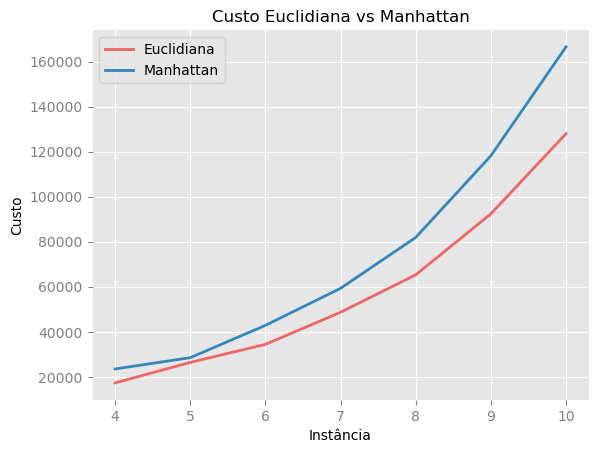
\includegraphics[width=9cm]{met_vs}
	\centering
\end{figure}

Para essa comparação, foi fixado o algoritmo como sendo o de Christofides. É possível perceber claramente que o custo da distância euclidiana é sempre menor que o custo da distância de Manhattan. Isso é esperado, pela definição dessas normas: vale que \( \textrm{dist}_{\textrm{Manhattan}}  \geq \textrm{dist}_{\textrm{euclidiana}} \). Para o TATT foi observado o mesmo comportamento.

\subsection{Tempo por distância}

Nesse caso, também foi fixado o algoritmo como sendo o de Christofides. Não houve diferença significativa entre os tempos de execução (nem para o TATT). De fato, o gráfico possui tempos tão semelhantes que optou-se por omiti-lo: sua visualização não agrega muito, e os dados podem ser consultados nas tabelas apresentadas anteriormente.

Um argumento que poderia favorecer o tempo da distância de Manhattan é o fato de ela trabalhar apenas com números inteiros, devido ao fato de as coordenadas dos pontos sempre serem inteiras também. Isso poderia facilitar eventuais cálculos, ao se evitar trabalhar com pontos flutuantes. Mas isso certamente não poderia ser um fator influente nesta implementação, porque optou por sempre representar as distâncias como \textit{floats}.

\subsection{Tempo por algoritmo}

Para essa comparação, assim como na próxima, foi fixado a métrica como sendo a distância euclidiana. Foi feito um ajuste na escala do gráfico: nesse caso é levado em consideração o \textit{tamanho} da instância propriamente dita, ao invés do expoente usado para gerar a instância, para trazer um melhor senso de escala e facilitar a visualização.

\begin{figure} [H]
	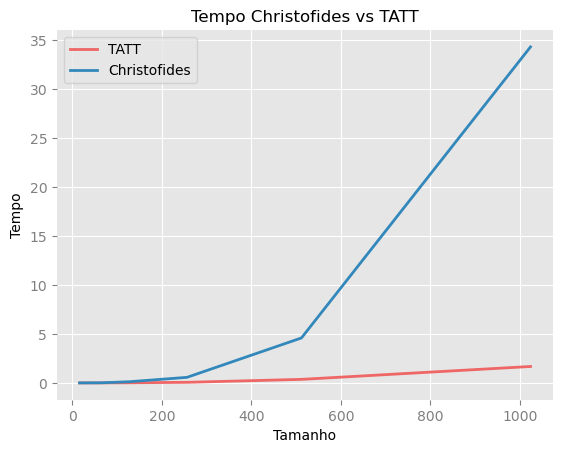
\includegraphics[width=9cm]{tempo_vs}
	\centering
\end{figure}

O TATT supera, e muito, o algoritmo de Christofides em termos de velocidade. Porém, isso é totalmente esperado. O custo do TATT é dominado pela computação da árvore geradora mínima (AGM). O algoritmo usado para computar a AGM, na \texttt{networkx}, é o algoritmo de Kruskal, cuja complexidade é \( \Theta(E \log V) \). Por outro lado, o custo do algoritmo de Christofides é consideravelmente maior, sendo dominado pela computação do \textit{matching} de peso mínimo. De acordo com a documentação da \texttt{networkx}, essa etapa é cúbica no número de vértices do grafo.

Apesar de não ter sido possível rodar \textit{branch and bound} em tempo hábil, vale à pena fazer um breve interlúdio. Comparando-se a custosa execução do BNB para \( n = 12 \) cidades, concluída em 28 minutos, com uma instância 80 vezes maior (\( n = 2^{10} \)) do TATT, necessitando apenas de um milésimo do tempo: apesar de aproximado, o TATT é muito mais viável na prática.

\subsection{Custo por algoritmo}

Apesar de compensar muito em tempo, o TATT \textit{pode} deixar a desejar em termos do ciclo encontrado. O custo obtido pelo algoritmo de Christofides é consistentemente menor. Novamente, esse resultado está totalmente dentro do esperado: o algoritmo de Christofides é 1.5 aproximado e o TATT é 2 aproximado. Na verdade, na prática, a média da proporção de custo até favoreceu o TATT: 1.17 (o esperado seria \( \approx 1.33 \)).

\begin{figure} [H]
	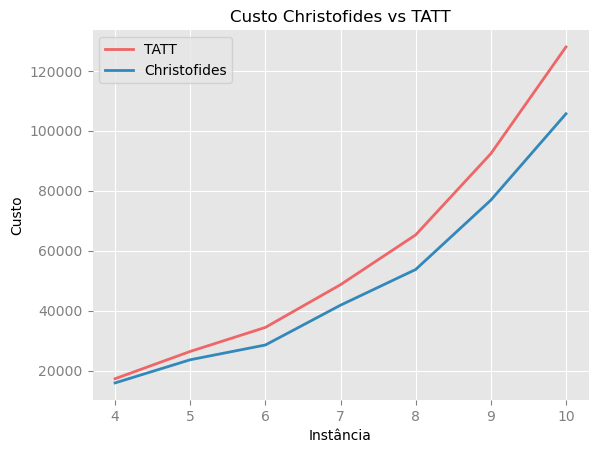
\includegraphics[width=9cm]{custo_vs}
	\centering
\end{figure}

\subsection{Memória}

Adicionalmente, também foi realizada uma análise do uso de memória, fazendo uso da biblioteca \texttt{memory\_profile}. Nessa análise, para os algoritmos de Christofides e \textit{Twice Around The Tree}, foi fixada uma instância de tamanho \( n = 2^{10} \), usando distância euclidiana. Para o \textit{branch and bound}, manteve-se a métrica, mas foi usada uma instância de tamanho \( n = 12 \).

\begin{figure} [H]
	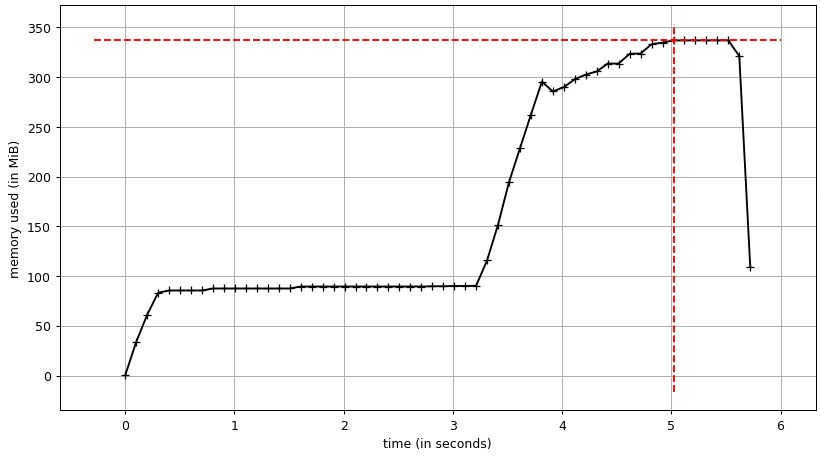
\includegraphics[width=9cm]{mem-tatt}
	\centering
	\captionsetup{labelformat=empty}
	\caption{Uso de memória para o TATT}
\end{figure}

O primeiro pico, logo no início do programa, se deve à inicialização, \textit{imports} e afins. O segundo pico, logo após os 3 segundos, corresponde à criação do grafo. Desde um pouco antes do \( t = 4s \), até o declínio final, o uso de memória é da função do algoritmo: sua subida ocorre devido à criação da AGM e, o breve período em que mantém constante corresponde ao caminhamento do grafo. O uso máximo de memória foi próximo de 340 MiB, aos 5 segundos.

\begin{figure} [H]
	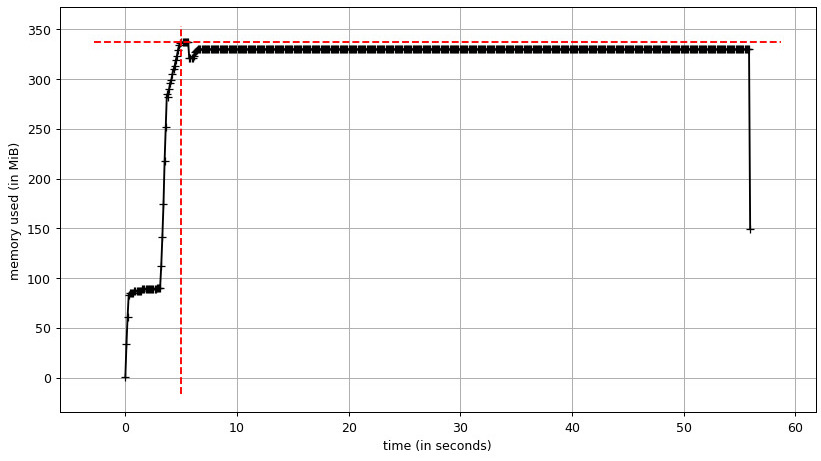
\includegraphics[width=9cm]{mem-chris}
	\centering
	\captionsetup{labelformat=empty}
	\caption{Uso de memória para o Christofides}
\end{figure}

É possível traçar um claro paralelo do uso de memória do Christofides e do TATT: o Christofides é uma versão ``esticada'' do TATT. Ambos possuem o pico de inicialização, da construção do grafo e da criação da AGM, mas como o Christofides é mais sofisticado, com algoritmos mais custosos, ele permanece mais tempo no estado de ``constância'', aos \( \approx \) 330 MiB.

\begin{figure} [H]
	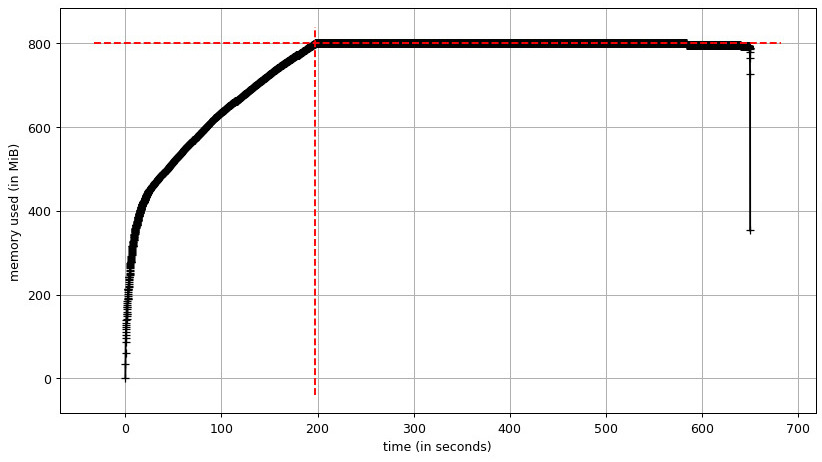
\includegraphics[width=9cm]{mem-bnb}
	\centering
	\captionsetup{labelformat=empty}
	\caption{Uso de memória para o BNB}
\end{figure}

O BNB, por outro lado, possui um perfil completamente diferente. Vale lembrar que a instância é 80 vezes menor, mas mesmo assim consumiu 2.35 vezes mais memória em seu pico. A maior parte dessa memória é alocada para criação de novos nós na árvore de busca, e pode variar muito dependendo da execução.

\section{Conclusão}

A principal lição aprendida com esse trabalho foi a inviabilidade dos algoritmos exponenciais. Especialmente pelo fato de o \textit{branch and bound} não ter apresentado o desempenho necessário, nem mesmo rodando para o limite inferior de tamanho de instância proposto, de \( n = 16 \). Em comparação, os algoritmos aproximativos fazem muito mais sentido para aplicações práticas, que podem escalar consideravelmente.

Em termos de implementação, foi realmente muito mais simples implementar o TATT e o algoritmo de Christofides. No entanto, isso não significa que desenvolver esses algoritmos não trouxe aprendizado nenhum. Pelo contrário: foi apenas passando por cada etapa que se tornou possível entendê-los por completo. Quanto ao BNB, houve mais desafio, mas também menos resultado. Certamente é possível otimizar a função de \textit{bound} para deixar o algoritmo viável pelo menos para a instância \( n = 16 \).

O trabalho também deu oportunidade de desenvolver diversas habilidades ``tangentes'', que não estão relacionadas ao propósito didático da atividade. Por exemplo, os testes usando o \texttt{pytest}, fazendo uso de \textit{fixtures} e com captura de exceções. Além disso, também foi um primeiro contato com a biblioteca \texttt{networkx}, que apresenta grande potencial para diversas aplicações. Outros primeiros contatos incluem o paralelismo e a biblioteca \texttt{numba}, em tentativas sem sucesso de otimizar o programa.

Em suma, o Trabalho Prático 2 da disciplina de Algoritmos II permitiu um aprofundamento maior no contexto de algoritmos exponenciais e aproximativos, possibilitado por meio de um contato mais íntimo com a linguagem de programação Python.

% \printbibliography

\end{document}
